\chapter{Experimental Apparatus}

While the Large Hadron Collider was approved over 20 years ago, much of its design was influenced by the needs of searches for physics beyond the Standard Model (BSM).
The two most important properties of a collider, for a BSM search, are its center-of-mass energy and its (instantaneous) luminosity, both of which were designed to be higher than any previous experiment. 
The designed center-of-mass energy ($\sqrt{s}$) of $14~TeV$ allows for the production of particles heavier than ever previously, while the designed luminosity of $10^{34}~cm^{-2}s^{-1}$ allows BSM searches to probe very rare processes.

In the same way, the design of the Compact Muon Solenoid (CMS) detector reflects the needs of BSM searches.
In particular, to fully search the uncovered parameter space of new physics an all-purpose, hermitic detector that can precisely measure a variety of particles and reliably determine the MET in an event is needed to cover the many (un)theorized new physics models.

This chapter summarizes in more detail the major features of both the LHC and CMS.
A complete description of both can be found in Refs.[include].

\begin{section}{The Large Hadron Collider}

The LHC since 2015 has been colliding protons together at $\sqrt{s} = 13~TeV$, slightly below the designed specifications but still at an unsurpassed energy.
In order to reach this center-of-mass energy, the LHC uses a large accelerator complex consisting of a sucession of many smaller particle accelerators, which is necessary to produce protons and bring them up to a speed such that they can be injected into the LHC ring.
A diagram of the CERN accelerator complex is shown in Figure~\ref{fig:lhc_accelerator_complex}.

\begin{figure}[tbp!]
\begin{center}
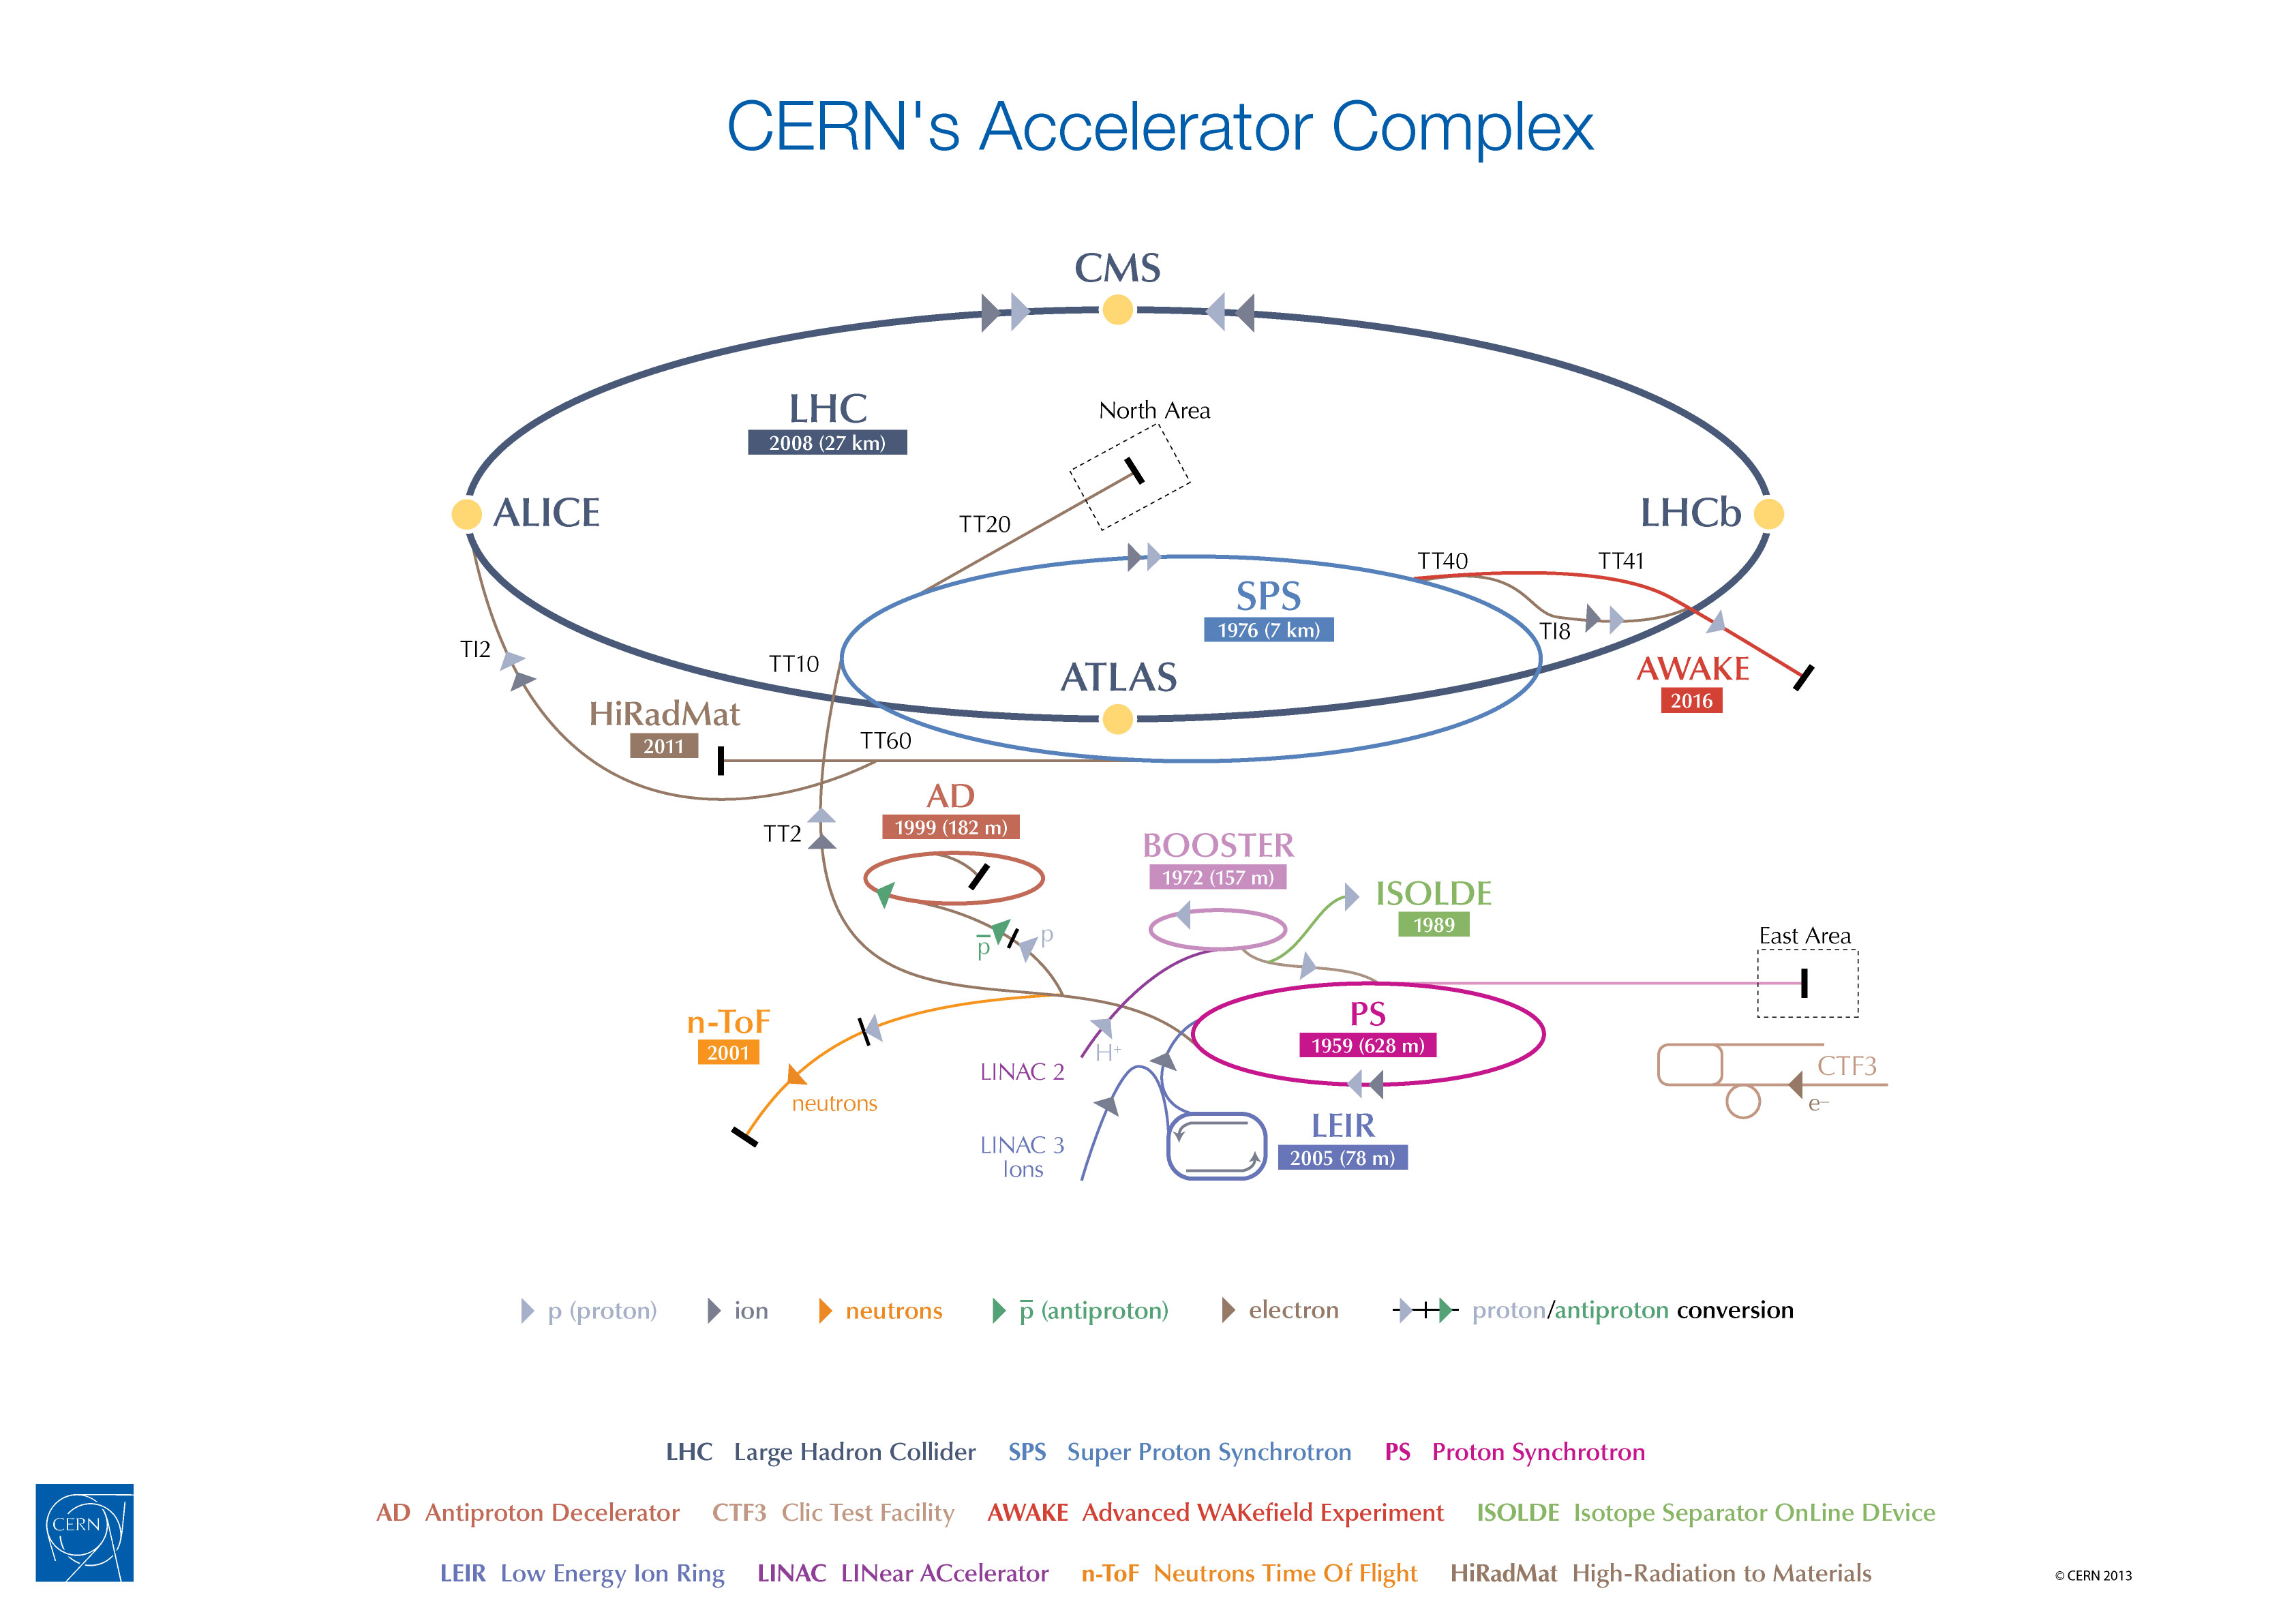
\includegraphics[angle=0,width=0.95\columnwidth]{fig/lhc_accelerator_complex.jpg}
\end{center}
\caption{A schematic of the CERN LHC accelerator complex.}
\label{fig:lhc_accelerator_complex}
\end{figure}

This process first begins with a simple bottle of hydrogen gas, which are ionized by an electric field to produce the needed protons.
These resulting protons are then fed into LINAC 2, the first accelerator in the chain, which accelerates them up to $50~MeV$, creating a beam of protons.
The proton beam is then passed succesively to the Proton Synchtron Booster, Proton Synchotron, and Super Proton Synchtron, where the beam reaches energies of $1.4~GeV$, $25~GeV$ and $450~GeV$, respectively.
At the Proton Synchotron, the beams are additionally split into ``bunches'', each consisting of $O(10^{11})$ protons and separated in time by 25~ns. 
Finally, the protons can be injected into the two beam pipes of the LHC, each circulating in opposite directions. 
These beams continue to be accelerated until they reach their final energy of 6.5 TeV, allowing for collisions at $\sqrt{s} = 13~TeV$.
At this point, the proton beams are focused and fine-tuned at several stages in order to increase the luminosity. 
In 2016, the LHC was able to collide protons with an instantaneous luminosity of $1.4~\times~10^{34}~cm^{-2}s^{-1}$, exceeding its designed specification, and deliver a record-high integrated luminosity of $41.07~fb^{-1}$.

These improvements from previous generations of colliders greatly increase the reach of searches for new, heavy particles.
Since the center-of-mass energy of the actual colliding partons ($\sqrt{\hat{s}}$) is typically much less than the overall center-of-mass energy, raising the collider's energy can greatly increase the production cross-section of heavy particles, especially of those around the TeV scale. 
For example, Figure~\ref{fig:parton_lumi}, which depicts the ratio of parton luminosities at $\sqrt{s} = 13~TeV$ and $8~TeV$ as a function of the characteristic mass scale of the event, shows that a $2000~GeV$ gluino will be produced through $gg$ scattering processes ${\sim}15\times$ more often with less than a doubling of the collider energy.
Increasing a collider's energy, however, is not always a practical option, involving new technologies, expensive upgrades, or even a new collider. When this is the case, the best alternative to continue to probe rare processes is to simply take more data, more quickly, which a high luminosity collider like the LHC allows for.


\begin{figure}[tbp!]
\begin{center}
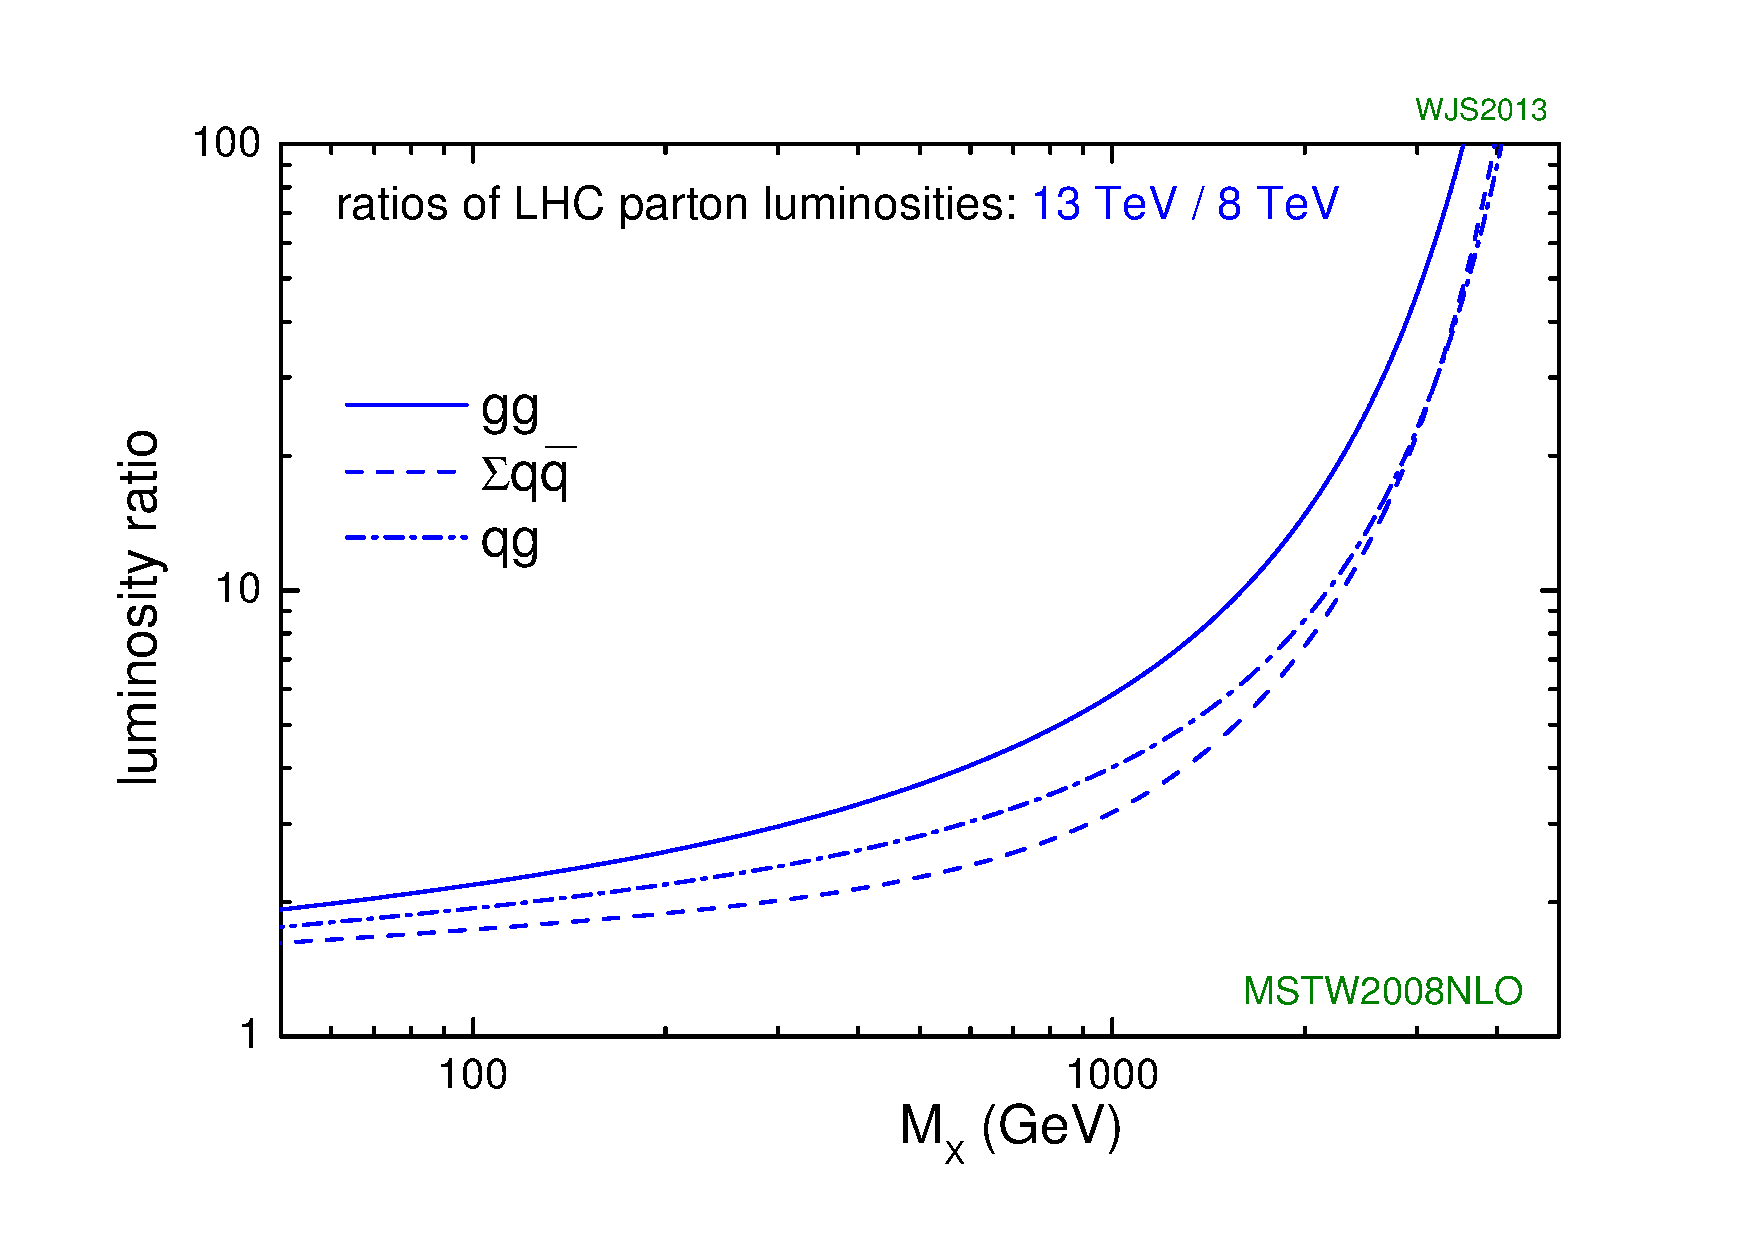
\includegraphics[angle=0,width=0.80\columnwidth]{fig/parton_lumi.pdf}
\end{center}
\caption{Ratio of parton luminosities at $\sqrt{s} = 13$ and $8~TeV$.}
\label{fig:parton_lumi}
\end{figure}


\end{section}

\begin{section}{Compact Muon Solenoid}

Along the tunnels of the LHC, below Cessy, France, sits the CMS detector where the proton-proton collisions are recorded.
The overall shape of the detector is cylindrical with a length of $21.6~m$ and radius of $7.3~m$, while weighing roughly 14,000 metric tons.  
The CMS detector is sometimes called a cylindrical onion, as this shape is constructed through layers of specialized detectors, each designed to provide precise measurements for a particular particle type.
Peeling back the layers from the outside-in, the first sub-detector is the muon system. 
Next is a superconducting solenoid of $6~m$ internal diameter that produces a magnetic field of $3.8~T$, and perhaps most importantly provides the ``S'' in CMS.
Placed within the solenoidal magnet, is the rest of the CMS detector, namely the Hadronical Calorimeter (HCAL), Electromagnetic Calorimeter (ECAL), and a silicon tracker.
The design of fitting most of the detector components within the solenoid is responsible for the ``C'' in CMS.
A diagram of the layout of the CMS detector can be seen in Figure~\ref{fig:cms_detector}.

\begin{figure}[tbp!]
\begin{center}
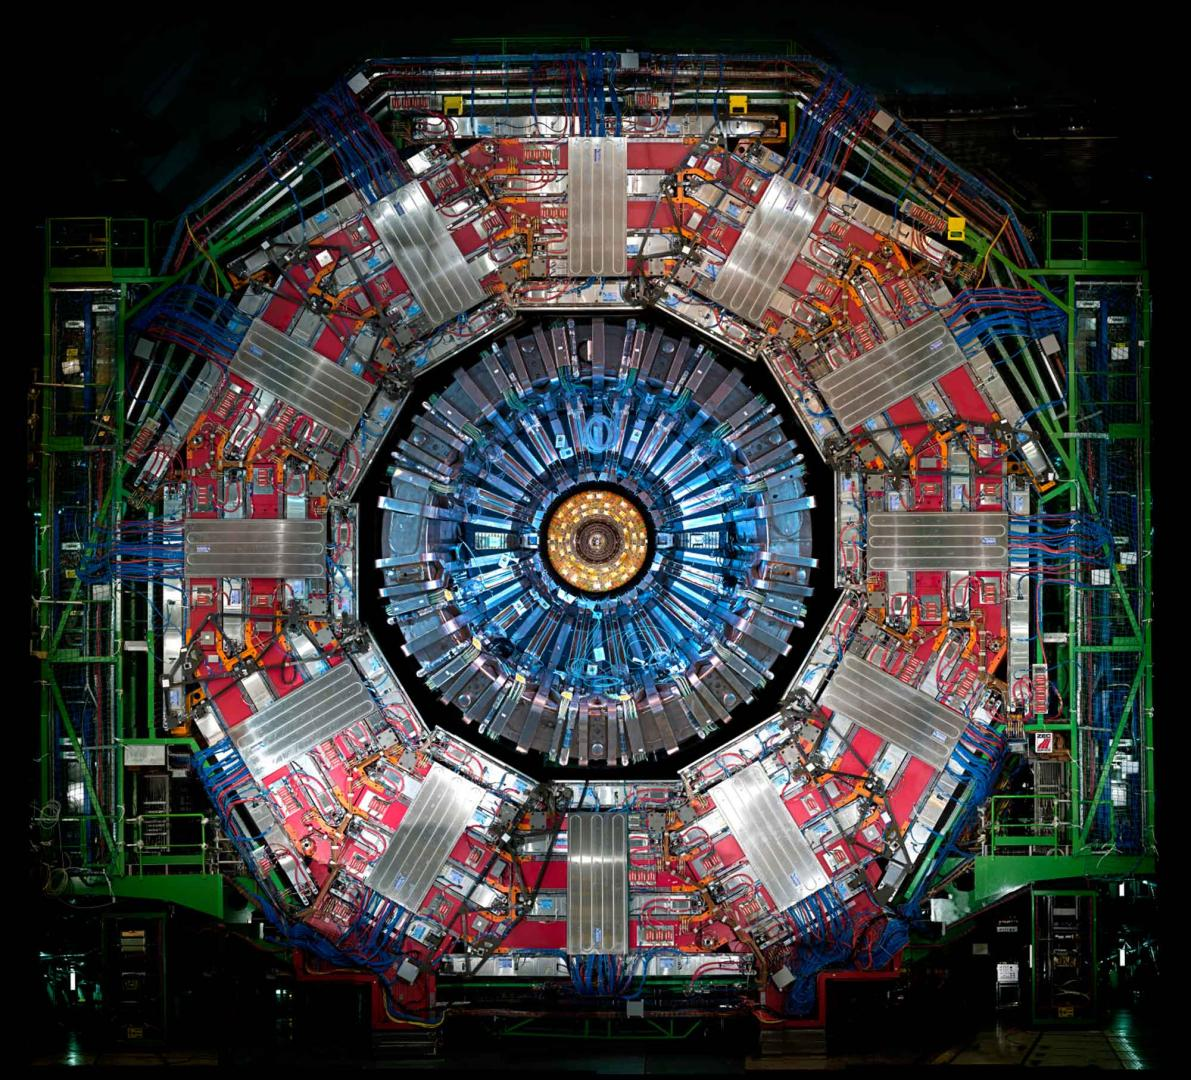
\includegraphics[angle=0,width=0.80\columnwidth]{fig/cms_detector.jpg}
\end{center}
\caption{A diagram showing the various sub-detectors of the CMS detector}.
\label{fig:cms_detector}
\end{figure}

At the center of the silicon tracker is Interaction Point 5, the beam crossing which provides the proton-proton collisions to the CMS detector, and is the nominal origin of CMS's coordinate system.
The $x$-axis is defined to point towards the center of the LHC ring and the $y$-axis is defined to point up towards the surface, both of which are transverse to the proton beam. 
The $z$-axis points along the beamline with the positive direction given by the right-hand rule relative to the $x$- and $y$-axes.
Due to CMS detector shape, it is often useful to convert the cartesian coordinates to a cylindrical coordinate system.
In this system, the azimuthal angle, $\phi$, is measured from the $x$-axis in the $xy$-plane, and the polar angle, $\theta$, is measured from the z-axis.
The polar angle, however, is often replaced by psuedorapidity, defined as $\eta = -\ln(\theta/2)$.
Thus, any point in the CMS coordinate system can be represented by $(z, \eta, \phi)$.
A diagram showing both the cartesian and cylindrical coordinate systems can be seen in Figure~\ref{fig:cms_coordinate_system}.

The remainder of this section briefly describes the meain features of the various CMS sub-detectors.

\begin{figure}[tbp!]
\begin{center}
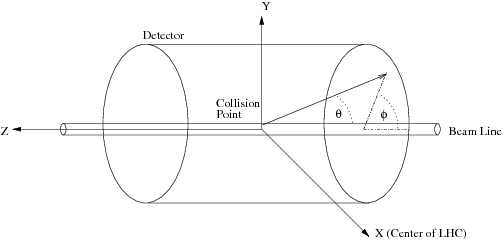
\includegraphics[angle=0,width=0.80\columnwidth]{fig/cms_coordinate_system.png}
\end{center}
\caption{A diagram of the cartesian and cylindrical coordinate systems used by CMS.}.
\label{fig:cms_coordinate_system}
\end{figure}

\begin{subsection}{Inner Tracking System}

The tracking system is used for precise measurements of the trajectories of charged particles, as well as reconstruction of seconday vertices.
As the tracking system is the closest subdetector to the interaction point, it faces a very large particle flux rate and so must be able to provide both high granularity and fast response, as well be able to survive operating in those conditions with ane expected lifetime of 10 years.
At the same time, these features must be balanced with minimizing the amount of material in order to reduce unwanted interactions with the detector, such as multiple scattering, photon conversion, and nuclear interactions.
These requirements lead to a tracking system composed entirely of silicon technology.

The CMS tracking system is actually composed of two parts.
The first is the pixel detector, which surrounds the interaction point, and is composed of 3 barrel layers at radii between $4.4$ and $10.2~cm$ and 2 endcap layers that extend the acceptance up to $|\eta|<2.5$.
In total, the pixel detector covers an area of roughly $1~m^{2}$ with 66 million pixels and achieves a resolution of roughly 10 and 20 microns in the directions transverse and logitudinal to the beam line, respectively.

The second part of the tracking system is the strips detector which sits just outside the pixel detector.
The strips detector is composed of 4 parts: the tracker inner barrel (TIB), tracker inner disks (TID), tracker outer barrel (TOB), and the tracker endcaps (TEC).
The TIB and TID extend up to $55~cm$ in radius and are composed of 4 and 3 layers, respectively, while the TOB, which surronds the TIB and TID, extends out to $116~cm$ and is composed of 6 layers.
Lastly, the TEC which sits next to the other strip detector components, covers a radius of 22.5 to $113.5~cm$ and is composed of 9 disks.
In total, the strips detector covers an area of $198~m^{2}$ with 9.3 million strips.
A layout of the tracking system including the pixel and strips detector is shown in Figure~\ref{fig:cms_tracker}.

\begin{figure}[tbp!]
\begin{center}
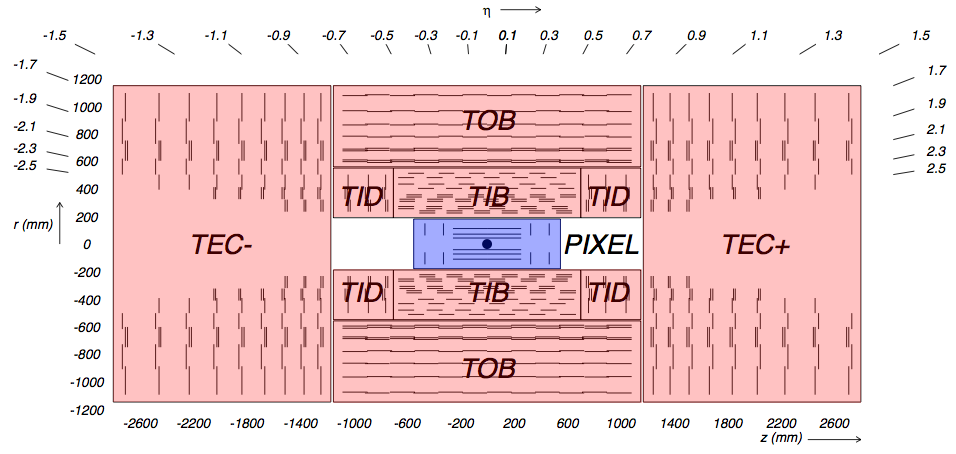
\includegraphics[angle=0,width=0.80\columnwidth]{fig/cms_tracker.png}
\end{center}
\caption{Layout of the CMS tracking system, showing both the pixel detector (blue) and the strips detector (red).}.
\label{fig:cms_tracker}
\end{figure}

\end{subsection}

\begin{subsection}{Electromagnetic Calorimeter}

The primary purpose of the electromagnetic calorimeter (ECAL) is to measure the energy of electrons and photons.
The ECAL is a hermetic, hemogenous detector made up of a barrel part, convering the $|\eta|<1.479$ region, and two endcap parts that covers $1.566<|\eta|<3.0$.
Both the barrel and endcap sections are comprised of lead tungstate ($PbWO_{4}$) crystals with 61,200 in the barrel and 7,324 in each of the endcaps.
The use of the $PbWO_{4}$ crystals was motivated by their high density, short radiation length, small Moli\`ere radius, and radiation hardness, all of which allow for a fine granularity, radiation resistant, compact calorimeter.

The lead tungstate crystals act as scintillators, which produce an amount of light that is proportional to the energy of an incident particle.
This light is then converted to an electrical signal by silicon photodectors (avalanche photodetectors in the barrel and vacuum hototriodes in the endcaps), which is used for the final energy measurement.
The resulting resolution on the energy measurements is given by 

\begin{equation}
\label{eq:ecal_resolution}
\frac{\sigma}{E} = \frac{S}{\sqrt{E}} \oplus \frac{N}{E} \oplus C
\end{equation}

where $S$ is the stochastic term, $N$ the noise term, $C$ the constant term, and $E$ is in units of $GeV$.
Typical values for $S$, $N$, and $C$, as measured in electron beam tests, are 2.8\%, 12\%, and 0.30\%, repectively.

In addition to the ECAL barrel and endcaps is a preshower detector, which sits in front of the endcaps, convering $1.653<|\eta|<2.6$.
The main purpose of the preshower detector is to identify neutral pions by improving the granularity, so as to be able resolve photon pairs from the decay of high energy pions that otherwise would be mis-measured as single photons. 
The preshower detector also provides improved position resolution for electrons and photons and helps identify electrons from minimium ionizing particles.
The full layout of the ECAL is shown in Figure~\ref{fig:cms_ecal}.

\begin{figure}[tbp!]
\begin{center}
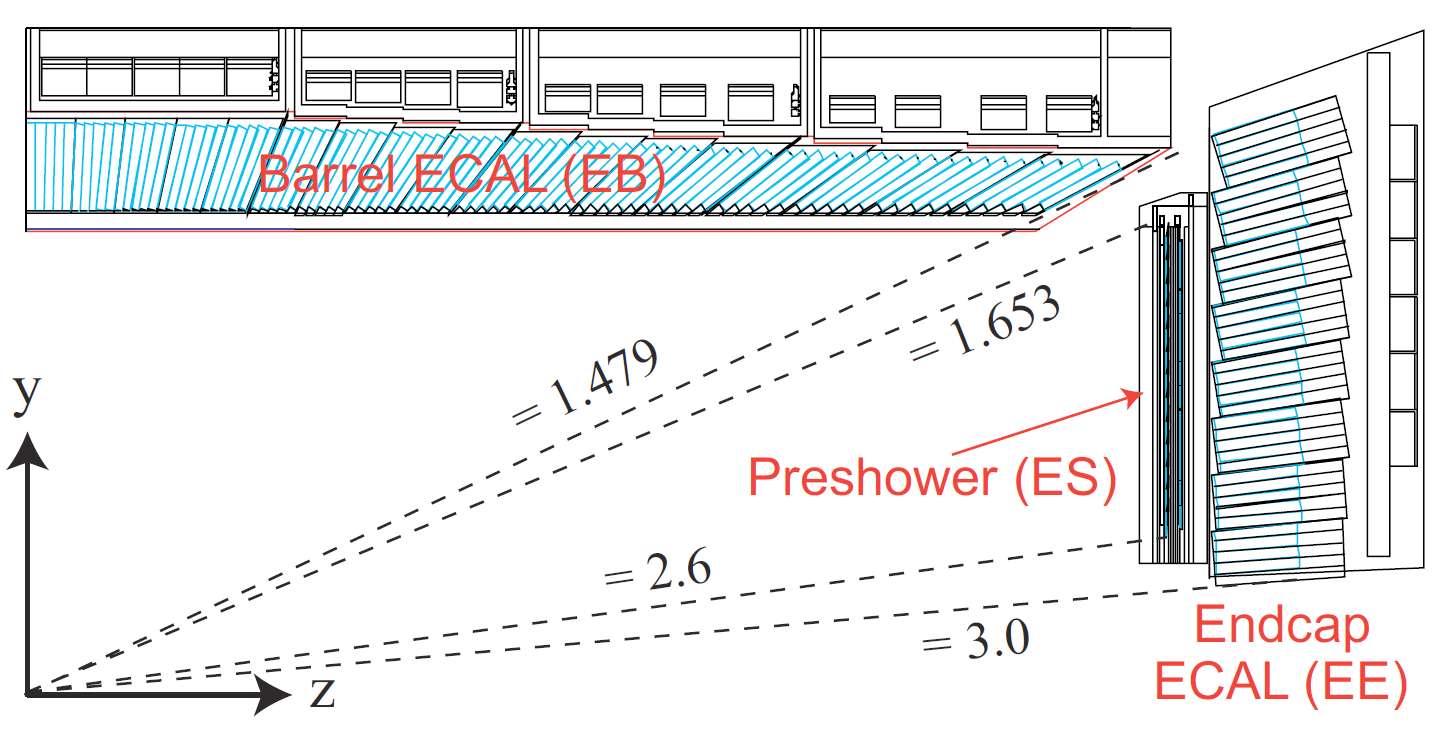
\includegraphics[angle=0,width=0.80\columnwidth]{fig/cms_ecal.png}
\end{center}
\caption{A cross section of the ECAL, showing its geometry and layout}.
\label{fig:cms_ecal}
\end{figure}

\end{subsection}

\begin{subsection}{Hadronic Calorimeter}

The primary purpose of the hadronic calorimeter (HCAL) is to measure the energy of hadrons, which can pass through the ECAL as they primarilly interact through the strong force.
The HCAL is a sampling calorimeter made up of either brass, iron, or steel absorbers and uses plastic scintillator tiles as the sampling material, which measures the energy of hadrons through scintillation, similarly to the ECAL:
As a hadron reaches through the HCAL, it interacts with one of the absorber layers, which results into a ``shower'' of particles that produces light in the scintillator tiles as the resulting particles pass through the sampling layers.
These light pulses are converted to electrical signals by optical fibers, which when summed have an amplitue proportional to the hadron's energy. 

\begin{figure}[tbp!]
\begin{center}
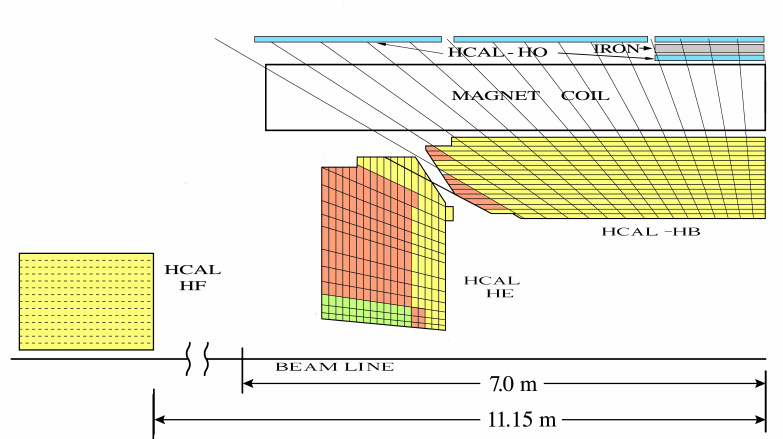
\includegraphics[angle=0,width=0.80\columnwidth]{fig/cms_hcal.png}
\end{center}
\caption{The layout and geometry of a quarter of the HCAL detector.}
\label{fig:cms_hcal}
\end{figure}

The HCAL is separated into 4 components: the hadron barrel (HB), hadron endcap (HE), hadron forward (HF), and hadron outer (HO), the layouts of which are shown in Figure~\ref{fig:cms_hcal}.
The HB and HE completely surround the ECAL and were designed to minimize any cracks between the two subdetectors with the HB covering $|\eta|<1.3$ and the HE covering the rest up to $|\eta|=3$.
Both components function as sampling calorimteres with alternating absorber and sampling layers.
In the HB, the first and last layers are made of steel while the 14 other absorber layers are made of brass, while the HE is made up of 18 brass absorber layers.
For both components, there are sampling layers made of plastic scintillator tiles interspersed between each of the absorber layers.

The HF is used to measure the energy of the forward most hadrons in the pseudorapidity range of $3.0<|\eta|<5.0$.
At this forward position, the HF faces extradorinary levels of particle flux and had to be designed to handle this radiation.
Due to this constraint, the HF uses quartz fibers instead of plastic scintillator tiles as its active medium, as the quartz fiber are more radiation hard.
The HF uses both long fibers, which run the full depth ($165~cm$) of the detector, and short fibers, which begin $22~cm$ from the front end of the detector.
This geometry allows the HF to provide depth information of the energy deposits, which helps to identify electron and photons from hadrons, as the former tends to deposit most of its energy in the first depth, while the latter deposits its energy more equally between the two depths.
These fibers are embedded into the steel structure of the HF, which also acts as the absorber.

Lastly is the HO, whose main purpose is to act as a ``tail catcher''. 
Due to the geometrical constraint that the HCAL fit within the CMS solenoid, the HB does not have enough material in the central $\eta$ region to adequately contain hadron showers.
So to provide extra sampling layers, the HO sits just beyond the solenoid and has 1 to 2 scintillator layers and uses the magnet as an extra absorber layer. 
At this position, the HO is able to identify late starting showers and measure the amount of energy that is deposited past the HB.

\end{subsection}

\begin{subsection}{Muon System}

Muons, as implied by the ``M'' in CMS, are a central focus of the CMS detector, and the responsibiilty of identifying muons with high purity and providing precise momenta measurements falls to the muon system.
To do this, the muon system is composed of three types of gaseous detectors, motivated by the need to cover a large area and varying radiation environments.
Figure~\ref{fig:cms_muonsys} shows the layout of the muon system within the CMS detector.

\begin{figure}[tbp!]
\begin{center}
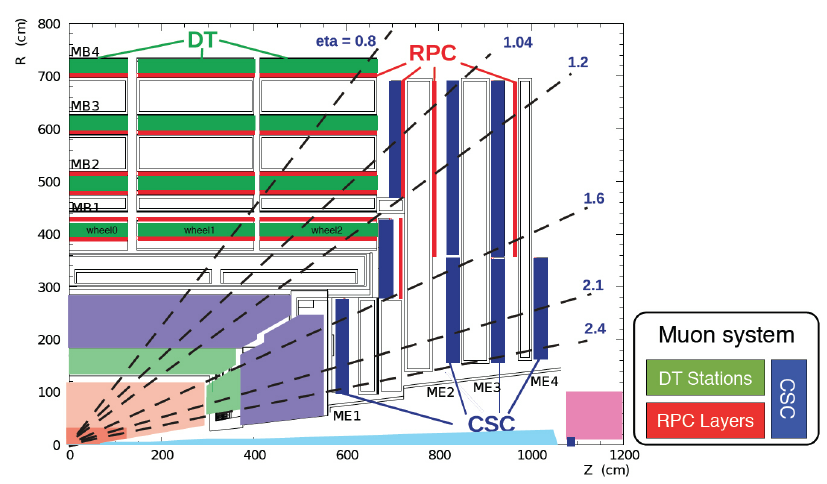
\includegraphics[angle=0,width=0.80\columnwidth]{fig/cms_muonsys.png}
\end{center}
\caption{The layout of the muon system within the CMS detector.}
\label{fig:cms_muonsys}
\end{figure}

In the barrel region, $|\eta|<1.2$, drift tube chambers (DTs) are used as the neutron-induced background is small, the muon rate is small, and the magnetic field is uniform.
The DTs are organized into 4 stations, with three of the stations containing 8 chambers that measure position in the $r-\phi$ plane and 4 that measure position in the $z$-direction.
The last station only contains the 8 $r-\phi$ measuring chambers.
In the endcap regions of CMS, $0.9<|\eta|<2.4$, the expected muon and background rates are higher and the magnetic field is large and non-uniform, both of which preclude the use of DTs.
Instead, the muon system endcaps are instrumented with cathode strip chambers (CSCs) that have a high response time, fine segmentation, and higher radiation resistance
The CSCs have 4 stations in each endcap with chambers that are aligned perpendicular to the beam line and are able to provide measurements in the $r-phi$ plane and $z$-direction, along with the beam crossing time of a muon.

Both the DTs and CSC are capable of providing high efficiency and pure muon $p_{T}$ triggers, independent of the rest of the detector.
But in order to further improve this, particularly at the full LHC luminosity, another complementary trigger system consisting of Resisitive Plate Chambers (RPCs) was added to both the the barrel and endcap regions ($|\eta|$<1.6).
The RPCs are double-gap chambers that operate with a fast response and good time resolution.
The spatial resolution, however, is coarser than the DTs or CSCs, though the extra hits in the RPC still help resolve ambiguities when making tracks.
There are a total of 6 RPC layers in the barrel muon system, which help improver triggers for low $p_{T}$ muons, and 3 layers in each of the endcaps that help reduce background and improve the time and $p_{T}$ resolution of muons.

\end{subsection}

\begin{subsection}{Trigger System}

The high instantaneous luminosity of the LHC provides many techincal challenges for the data aquisition system (DAQ), with proton-proton collissions occuring every $25~ns$, corresponding to a frequency of $40~MHz$. 
At this collision rate, it is unfeasible to process and store the data for each event.
In order to reduce the rate, a two-stage trigger system is used to select only the most ``interesting'' events for processing.

The first stage is the Level-1 (L1) trigger system, which has approximately only $4~\mu$s to decide whether or not an event should be further processed. 
In order to operate at this timescale, the L1 trigger uses only coarse-grained information from the CMS calorimeters and the muon system.

For the calorimeter set of data, the L1 first generates trigger primitives by looking for lar for large energy deposits in the calorimter.
These trigger primitives are then passed to the Regional Calorimeter Trigger (RCT), which uses this information to determine electron/photon candidates and transverse energy sums per calorimeter region.
In addition, the RCT also calculates information relevant for detecting minimally ionizing particles, vetoing tau leptons, and muon isolation.
Lastly, the Global Calorimeter Trigger (GCT) uses the information from the RCT to construct jets and calculate the event-level transverse energy and missing transverse energy, along with the final isolated and non-isolated electron/photon candidates.

For the muon portion of the L1 trigger system, the DTs and CSCs both compute local trigger informationwhich consists of two- and three-dimensional track segments, respectively.
This information is then passed to a join DT-CSC track finder, which connects these segments into a full candidate track.
At the same time, the RPC constructs a separate, independent set of track candidates.
Both sets of candidate tracks are sent to the Global Muon trigger (GMT), which also takes in the relavent information from the RCT), to construct muon candidates.

Lastly, the candidate particles and event-level information from the GCT and GMT are sent to the Global Trigger, which takes this information and checks to see if certain criteria are met.
If so, a L1 Accept (L1A) is generated, which signals for the event to be fully read out.
This process, shown in Figure~\ref{fig:cms_trigger}, reduces the full readout rate to at most $100~kHz$.

\begin{figure}[tbp!]
\begin{center}
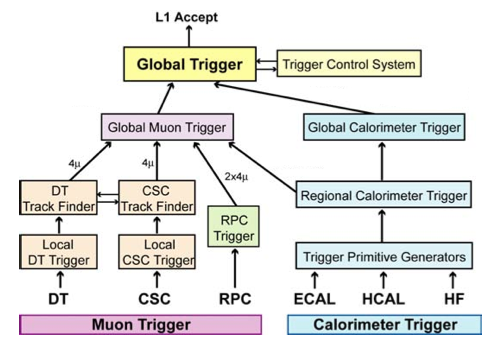
\includegraphics[angle=0,width=0.80\columnwidth]{fig/cms_trigger.png}
\end{center}
\caption{Flowchart depicting the generation of a L1 Accept.}
\label{fig:cms_trigger}
\end{figure}

On the generation of an L1A, all the CMS subsystems read out their buffered data corresponding to the L1A event to the an event builder.
The data the event builder receives is both more complete and at a finer resolution, allowing it to construct more complex quantities before sending it to the High Level Trigger (HLT), the second stage of the trigger system.

The HLT software is run on a processor farm that reconstructs events in greater detail to decide whether or not they should be kept.
This framework is flexible as both the HLT software and the processor farm can be updated to meet changing experimental needs.
As such the exact criteria used by the HLT in its decision varies with time, but generally involves thresholding the $p_{T}$ and/or multiplicity of particles along with event-level quantities, such as $H_{T}$.
At the end of this process, the trigger rate is at approximately $100~Hz$.

\end{subsection}

\end{section}



%Notes:
% Add a physical view of the LHC (like a map view)
% Add proper TeV/GeV/MeV commands and fb-1
% pT, HT
% Can expand by talking about how the beam is squeezed.
% Add references
% Add an HF timing section

%References:
% https://home.cern/about/accelerators
% https://cds.cern.ch/record/1621583 (acclerator complex)
% tdr
% http://iopscience.iop.org/article/10.1088/1748-0221/3/08/S08004/meta (CMS JINST)
% http://inspirehep.net/record/1236817/plots
